% Copyright (C)  2015  Alexander Jankowski, Philipp Hacker.
% Permission is granted to copy, distribute and/or modify this document
% under the terms of the GNU Free Documentation License, Version 1.3
% or any later version published by the Free Software Foundation;
% with no Invariant Sections, no Front-Cover Texts, and no Back-Cover Texts.
% The lincense itself can be found at <https://www.gnu.org/licenses/fdl-1.3>.

\documentclass[numbers=noenddot,a4paper,notitlepage,twoside,BCOR15mm]{scrartcl}
%\documentclass[numbers=noenddot,12pt,a4paper]{scrartcl}

\usepackage{ifoddpage}
\usepackage[infoshow]{tabularx}
\usepackage{fancyhdr}
\usepackage[greek,ngerman]{babel}
\usepackage[T1]{fontenc}
\usepackage[utf8]{inputenc}
\usepackage{libertine}
\usepackage{ziffer}
\usepackage{graphicx}
\usepackage{units}
\usepackage[infoshow]{tabularx}
\usepackage[all]{xy}
\usepackage{amsmath}
\usepackage{amssymb}
\usepackage{wrapfig}
\usepackage{upgreek}
\usepackage{esint}
\usepackage{float}
\usepackage[font=small,labelfont=bf]{caption}
\usepackage{subcaption}
\usepackage{lscape}
\usepackage[backref=page]{hyperref}
\usepackage{cleveref}
\usepackage{csquotes}

\renewcommand{\headrulewidth}{0.1pt}
\renewcommand{\footrulewidth}{0.1pt}
\newcommand{\name}{\text{Name}} %TODO Name des Protokollanten eintragen

\renewcaptionname{ngerman}{\figurename}{Abb. }
\renewcaptionname{ngerman}{\tablename}{Tab.}

\setlength{\parindent}{0pt}

\newcommand{\nummat}[1]{\left[\text{#1}\right]}
\newcommand{\num}[1]{$\left[\text{#1}\right]$}
\newcommand{\degree}{^\circ}
\newcommand{\diff}{\textnormal{d}}
\newcommand{\tenpo}[1]{ 10^{#1}}
\newcommand{\greek}[1]{\greektext#1\latintext}
\newcommand{\ix}[1]{_\text{#1}}
\newcommand{\imag}{\mathbf{i}}
\newcommand{\tilt}[1]{\textit{#1}}
\newcommand{\grad}[1]{\textit{grad}\left(#1\right)}
\newcommand{\divergenz}[1]{\textit{div}\left(#1\right)}
\newcommand{\euler}{\mathnormal{e}}
\newcommand{\fett}[1]{\textbf{#1}}
\newcommand{\einnup}{\hspace{0.2cm}}
\newcommand{\einnum}{\hspace{-0.2cm}}
\newcommand{\zentriert}[1]{\begin{center}#1\end{center}}

\title{Protokoll: Versuch} %TODO Name des Versuchs eintragen
\author{Alexander Jankowski, Philipp Hacker}
\date{\today}
\pagestyle{fancy}
\fancyhead[C]{\thepage}
\fancyhead[R]{\name}
\fancyfoot[C]{\thepage}
\fancyhead[L]{Abschnitt \thesection}

\begin{document}
	\maketitle
	\begin{center}
		Betreuer: \\ %TODO Name des Betreuers eintragen
		Versuchsdatum: \\ %TODO Datum des Versuchs eintragen
		\begin{table}[h]
			\centering
			Note: %TODO Gute Note erhalten :)
			\begin{tabularx}{1.5cm}{|X|}
				\hline \\ \\
				\hline
			\end{tabularx}
		\end{table}
	\end{center}
	\vspace*{\fill}
	\tableofcontents
	\vfill
	\clearpage
	\section{Motivation}

		Ionenfallen werden in der modernen Physik in sehr vielen Bereichen verwendet. Man nutzt sie als Hilfen in der Massenspektrometrie, für die Analyse von Eigenschaften geladener Nanoteilchen oder zur Erzeugung und Manipulation von komplexeren Molekülen. Insbesondere in der Cluster-Physik sind Fallen der wichtigste Bestandteil in der Methodik. Dabei greift man auf Kombinationen von elektrostatischen, magnetischen oder Wechselfeldern in einem endlichen, meist sehr kleinen Raumbereich , welcher verschiedenste, dem Problem angepasste Geometrien vorweist, zurück. Im Rahmen dieses Versuches sollen die Speichereigenschaften von Stickstoff-Ionen in einer hyperbolischen Paul-Falle untersucht werden. 


	\clearpage
	\section{Physikalische Grundlagen}

		Bei einer sogenannten \tilt{Paul-Falle} handelt es sich um eine zylindersymmetrische Ionenfalle, welche über komplexe elektrische Wechselfelder in ihrem Inneren den Einfang und die Speicherung von geladenen Partikeln, e.g. Ionen ermöglicht. Die physikalischen Grundlagen und Beispiele folgen in diesem Abschnitt.

		\subsection{Speicherung, Stabilität und Dynamik}

				\begin{wrapfigure}{r}{0.4\textwidth}
					\centering
					\vspace{-0.5cm}
					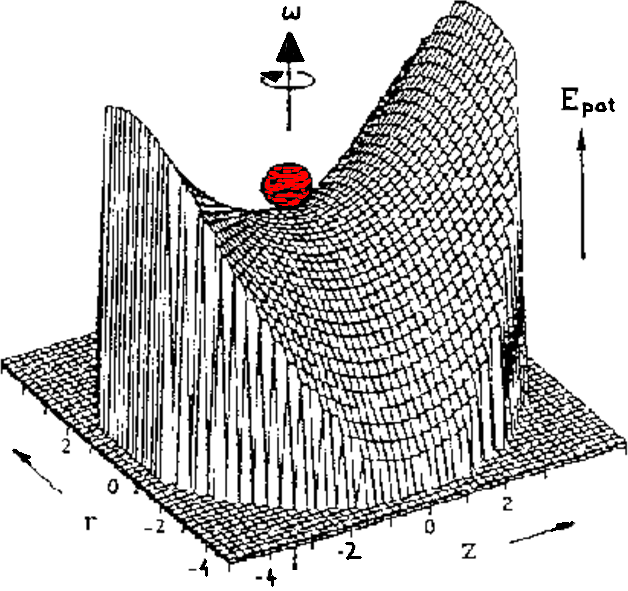
\includegraphics[width=0.4\textwidth]{paulpotential.png}
					\caption{Mit der Frequenz $\omega$ durch ein hamonisches, elektrostatisches Einfangpotential gyrierendes, geladenes Teilchen. \cite{UMainzReflektron}}\label{img:potential}
				\end{wrapfigure}

			Ein Teilchen ist in einem elektrostatischen Potential genau dann gefangen, wenn eine rücktreibende Kraft $\vec{F}\propto-\vec{r}$ auf diese aus allen Richtungen wirkt. Mit der \tilt{Laplace-Gleichung} für ein radial-symmetrisches Problem entlang einer 'Zylinderachse' $\vec{e}\ix{z}$ folgt das harmonische Speicherpotential $\Phi(x,y,z)$ in \autoref{eq:pot}, welches der Form in \autoref{img:potential} im Allgemeinen entspricht. Man gestaltet den Aufbau günstiger Weise so, dass Oberflächen innerhalb der Falle den Äquipotentialflächen von $\Phi(x,y,z)$ entsprechen, weswegen für die Endkappen (\fett{links}) und die Ringelektrode selbst (\fett{rechts}) die Geometriegleichungen in \autoref{eq:geome} gelten. Einen schematischen, verallgemeinerten Aufbau zeigt \autoref{img:schem_aufbau}.

				\begin{align}
					\Phi(x,y,z)=\frac{\Phi\ix{0}}{\gamma}(x^2+y^2-2z^2) \label{eq:pot} \\
					x^2+y^2-2z^2=-2z\ix{0}^2 \quad\text{und}\quad x^2+y^2-2z^2=r\ix{0}^2 \label{eq:geome}
				\end{align}

				\begin{figure}[t]
					\centering
					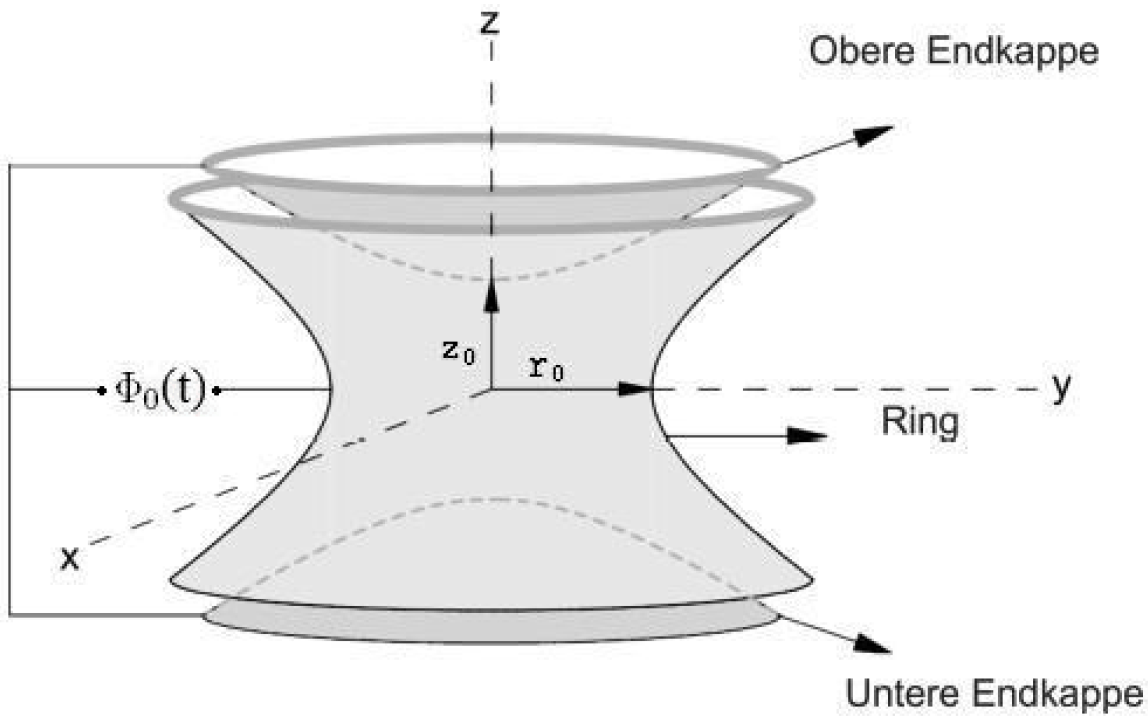
\includegraphics[width=0.6\textwidth]{paul_schema.png}
					\caption{Schematischer Aufbau einer Paul-Falle mit radialsymmetrischer Geometrie. Hyperbolische Formen als Äquipotentialflächen. \cite{EMAUGreifswaldPaul}}\label{img:schem_aufbau}
				\end{figure}

		Hierbei wird der charakteristische \tilt{Fallendimensionsparameter} $d\ix{0}=\sqrt{\gamma/2}=\sqrt{r\ix{0}^2/2+z\ix{0}^2}$ definiert. Um in $\Phi(x,y,z)$ ein ideales Quadrupolfeld zu erreichen, wählt man $r\ix{0}=\sqrt{2}z\ix{0}$.\\
		Als Konsequenz des Earnshaw-Theorems benötigt es eine Überlagerung von elektrostatischen und wechselnden Feldern in der Paul-Falle, um eine Speicherung im Zentrum zu erreichen \cite{EarnPaul} \cite{Paul}. Nimmt man die Gleichspannung $U\ix{0}$ und überlagert sie mit einer Wechselspannung der Amplitude $V\ix{0}$ und Frequenz $\Omega/2\pi$, so erhält man das neue Speicherpotential \autoref{eq:neupot}. Man spricht bei $V(t)$ auch vom sogenannten Führungsfeld, da dieses maßgeblich die Teilchenbewegungen in der Falle beeinflusst.

			\begin{align}
				\Phi(x,y,z)=\frac{U\ix{0}+V\ix{0}\cos(\Omega t)}{2d\ix{0}^2}(x^2+y^2-2z^2) \label{eq:neupot}
			\end{align}

		Über die \tilt{newtonsche Bewegungsgleichung} $m\ddot{\vec{x}}=-q\vec{\nabla}\Phi$ und den dimensionslosen Variablen $\tau$, $a\ix{i}$ und $q\ix{i}$ aus \autoref{eq:param} ergeben sich die \tilt{Mathieuschen Differentialgleichungen} für die Bewegung eines mit $q$ geladenen Teilchens in kanonischer Form in \autoref{eq:mathieu}.

			\begin{align}
				\tau=\frac{\Omega t}{2} \quad \text{und} \quad q\ix{z}=\frac{4qV\ix{0}}{md\ix{0}^2\Omega^2}=-2q\ix{x}=-2q\ix{y} \label{eq:param}\\
				a\ix{z}=-\frac{8qU\ix{0}}{md\ix{0}^2\Omega^2}=-2a\ix{x}=-2a\ix{y} \nonumber \\
				0=\frac{\diff^2x\ix{i}}{\diff\tau^2}+\left(a\ix{i}-2q\ix{i}\cos(2\tau)\right)x\ix{i} \label{eq:mathieu}
			\end{align}

		Diese nichtlinearen Differentialgleichung 2. Ordnung haben die Lösungen $x\ix{i}(\tau)$, welche sich über die Parameter der Anfangsbedingungen $\gamma\ix{1,2}$, eine komplexe Konstante $\mu\ix{i}$ und eine $\pi$-periodische Funktion $\phi$ als Linearkombinationen zweier anderer Lösungen schreiben lassen (\autoref{eq:lös}.\\
		Schreibt man $\mu\ix{i}=\imag\beta\ix{i}$ um, so kann man einen Kettenbruch nach \cite{Bruch} und \cite{Bruch2} wie in \autoref{eq:bruch} annähern.

			\begin{align}
				x\ix{i}(\tau)=\gamma\ix{1}\exp(\mu\ix{i}\tau)\phi(\tau)+&\gamma\ix{2}\exp(-\mu\ix{i}\tau)\phi(-\tau) \label{eq:lös} \\
				\beta\ix{i}=a\ix{i}-\frac{(a\ix{i}-1)q\ix{i}^2}{2(a\ix{i}-1)^2-q\ix{i}^2}-\frac{(5a\ix{i}+7)q\ix{i}^4}{32(a\ix{i}-1)^3(a\ix{i}-4)}&-\frac{(9a\ix{i}^2+58a\ix{i}+29)q\ix{i}^6}{64(a\ix{i}-1)^5(a\ix{i}-4)(a\ix{i}-9)} \label{eq:bruch}
			\end{align}

		Kombinationen von $a\ix{i}$ und $q\ix{i}$ sind genau dann eine stabile Speicherung eines Teilchens, wenn sie die DGL's \autoref{eq:mathieu} und die Näherung \autoref{eq:bruch} erfüllen. Zu beachten ist dabei, dass in die benutzten Parameter Masse, Ladung sowie die verschiedenen Größen und Dimensionen der Paul-Falle eingehen. Daher ist es von besonderer Bedeutung, die Stabilitätsbereiche, wie sie in \autoref{img:stab} für $a\ix{z},q\ix{z}$ gezeigt werden, für die Probesubstanz zu kennen.

			\begin{figure}[t]
				\centering
				\begin{subfigure}[t]{0.4\textwidth}
					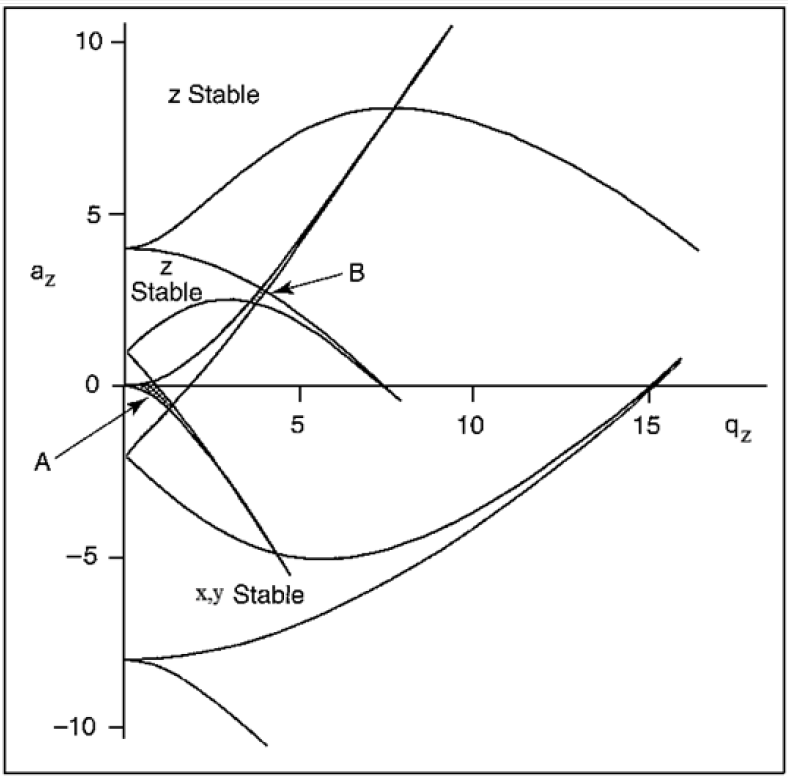
\includegraphics[width=\textwidth]{stab_1.png}
					\caption{}\label{img:stab1}
				\end{subfigure}
				\vspace{0.2cm}
				\begin{subfigure}[t]{0.37\textwidth}
					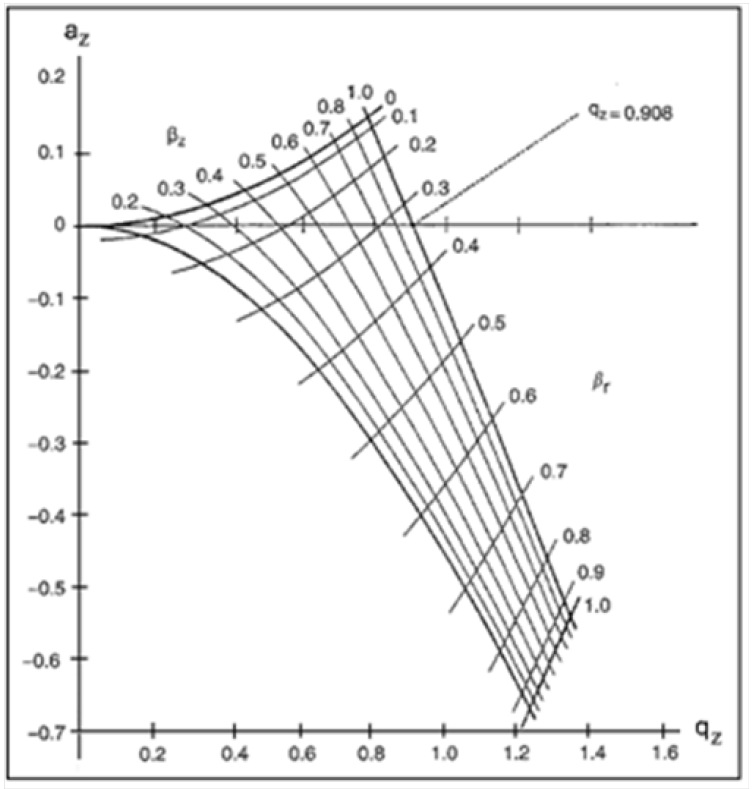
\includegraphics[width=\textwidth]{stab_2.png}
					\caption{}\label{img:stab2}
				\end{subfigure}
				\caption{\fett{(a):} $a\ix{z}$ gegen $q\ix{z}$. Überlappungen der Graphen sind Gebiete dreidimensionaler Speicherung. \fett{(b):} Vergrößerung des Bereiches A aus \fett{(a)}. Eingezeichnet sind die Linien gleichen $\beta\ix{z}$ und $\beta\ix{r}$. }\label{img:stab}
			\end{figure}


			\paragraph{Bewegungresonanzen}

				Mit der Fourier-Reihenentwicklung in \autoref{eq:fourie} der ursprünglichen \autoref{eq:lös} erhält man das Eigenfrequenzspektrum der Teilchenbewegungen in einer Paul-Falle. Die Koeffizienten $A=\gamma\ix{1}+\gamma\ix{2}$, $B=\imag(\gamma\ix{1}+\gamma\ix{2})$ und die der Reihen für Sinus und Cosinus $C\ix{2n,i}$ hängen von unseren Parametern $(a\ix{i},q\ix{i})$ ab und konvergieren für große $n$ schnell gegen 0, weswegen argumentiert werden kann, dass höhere Eigenfrequenzen weniger stark in das Spektrum einfließen. Beachtet man nur $n=0,\pm1$ so erhält man die Bewegung eines geladenen Partikels in der Paul-Falle in \autoref{eq:beweg}.

					\begin{align}
						x\ix{i}(\tau)=A\sum_{n=-\infty}^{\infty}C\ix{2n,i}\cos[(2n\pm\beta\ix{i})\tau]+B\sum_{n=-\infty}^{\infty}C\ix{2n,i}\sin[(2n\pm\beta\ix{i})\tau] \label{eq:fourie} \\
						x\ix{i}(\tau)=\sqrt{A^2+B^2}C\ix{0,i}\left[1-\frac{q\ix{i}}{2}\cos(\Omega t)\right]\cos\left[\frac{\beta\ix{i}}{2}\Omega t-\arctan\left(\frac{B}{A}\right)\right] \label{eq:beweg}
					\end{align}

			Die erste $\left[\dots\right]$ entspricht der sogenannten \tilt{Makrobewegung} mit der Frequenz $\omega\ix{i}=1/2 \beta\ix{i}\Omega$, die zweite $\left[\dots\right]$ der \tilt{Mikrobewegung} mit $\omega=\Omega$. Die Amplitude letzterer wird dabei maßgeblich durch die der Makrobewegung, also des Führungsfeldes beeinflusst.\\
			Geht man wieder auf die ursprüngliche, vollständige Fourier-Reihe der Bewegung mit dieser Kenntnis ein, so kann man das vollständige Eigenfrequenz-Spektrum der Makroschwingungen eines Teilchens in einer Paul-Falle mit \autoref{eq:spektr} beschreiben. Aus dieser Herleitung ergeben sich wichtige experimentelle Möglichkeiten: die resonante Anregung von gespeicherten Teilchen durch Energieaufnahme aus einem, in geeigneter Weise gerichteten, frequentierten zusätzlichen Feldes. Auf diese Weise erhöht sich der Bahnradius der Gyration und ein Teilchen kann austreten bzw. auf die Fallen-Elektroden treffen.

				\begin{align}
					\omega\ix{n,i}=\frac{(2n\pm\beta\ix{i})\Omega}{2} \label{eq:spektr}
				\end{align}

			\begin{figure}
				\centering
				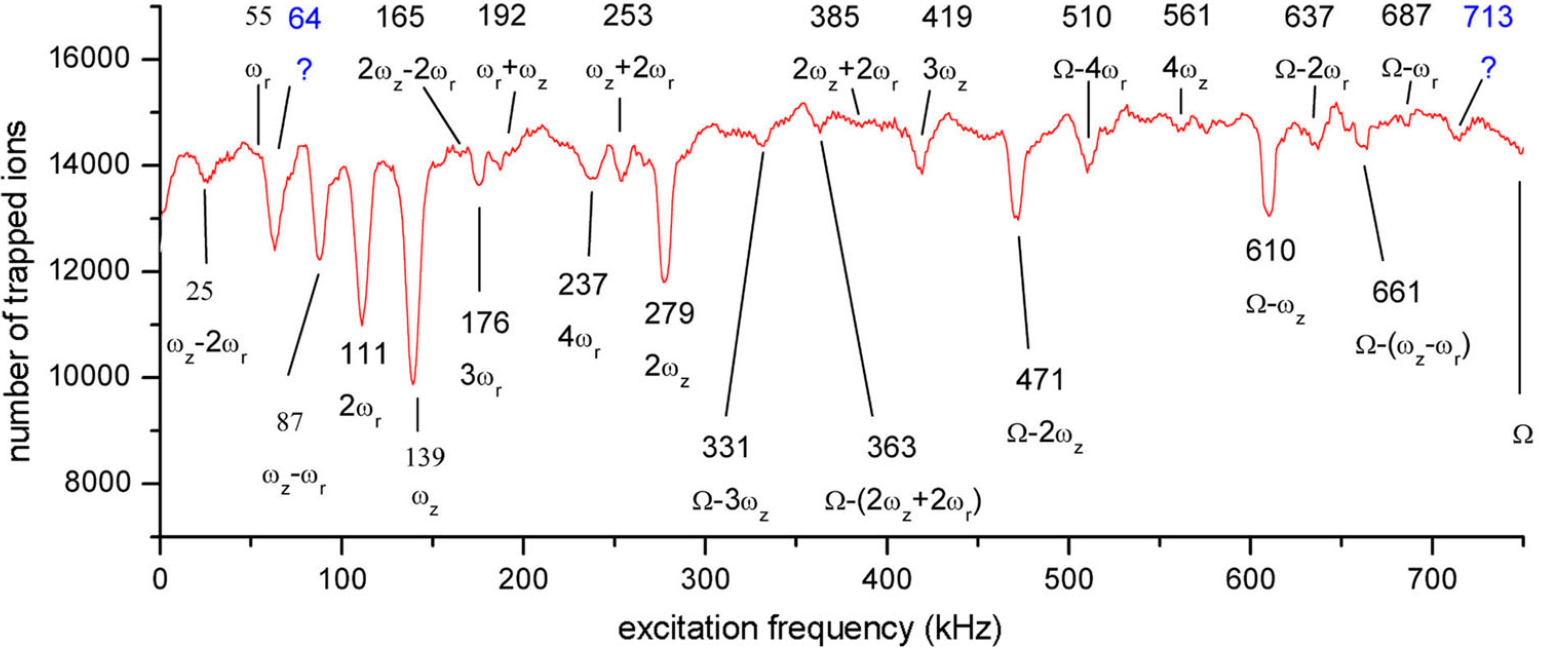
\includegraphics[width=\textwidth]{referenz.png}
				\caption{Literatur-Spektrum aus \cite{Paul-FalleREF} für $\fett{N}_2$-Ionen. Angetragen sind die jeweiligen Resonanzfrequenzen für die Differenz aus Signalen einer Referenz ohne und mit Anregung.}\label{img:referenz}
			\end{figure}

		\subsection{Arten von Ionenfallen}

			Ionenfallen werden im Allgemeinen nach ihrer Methodik und dem Ziel der Untersuchungen, welche damit durchgeführt werden, kategorisiert. Im folgenden sollen kurz einige (wichtige) Typen vorgestellt werden.

				\paragraph{Quadrupol-Ionenfallen}
					Bei Quadrupol-Fallen handelt es sich im allgemeinen um Paul-Fallen: die Überlagerung des Potentials von Gleich- und Wechselspannungsanteilen von 4 unterschiedlich angeordneten Elektroden ermöglicht den Einschluss einer ausgewählten $m/q$-Spezies innerhalb des Aufbaus. Zusätzlich benutzt man Endkappen, welche der Abstoßung dienen und einen axialen Einschluss sichern.\\
					Eine \fett{planare} 2D-Quadrupol-Falle hat ein zusätzliches Randfeld, um die Ionen einzufangen. Die ebene Anordnung hat eine erhöhte Speicherkapazität im Vergleich zu dem Aufbau dieses Versuch.\\
					Die \fett{lineare} Falle erweitertet den vorherigen Fall um eine Dimension entlang der Symmetrie-Achse. Wiederum sorgen Endkappen wieder für den axialen Einfang. Sie wird oft als selektiver Massenfilter benutzt.\\
					Eine \fett{hyperbolische} Paul-Falle liegt in diesem Experiment vor. Den Aufbau sieht man in \autoref{img:aufbau}. Unter anderem werden solche Geräte als Miniatur-Massenspektrometer und in medizinischen Anwendungen benutzt.\\
					Generell sind die Vorteile dieser Methode die hohe Empfindlichkeit, die kompakte Form und vergleichsweise hohe speicherbare Massen. Nachteilig sind die auftretenden Raum-Ladungs-Effekte bei hohen Strömen in und aus der Falle heraus sowie die nichtlinearen Resonanzen

				\paragraph{Penning-Falle}
					In der Penning-Falle werden die geladenen Teilchen in einem homogenen Magnetfeld auf Kreisbahnen gezwungen. Das zusätzliche elektrische Quadrupol-Feld verhindert, dass sich die Teilchen entlang der Magnetfeldlinien aus der Falle bewegen. Auf der Fallen-Achse verhindern statisch geladenen Endkappen durch Abstoßung das Austreten der Probesubstanz.\\
					Im Allgemeinen besteht eine Penning-Falle aus einer Ringelektrode und zwei Endkappen, wobei diese das gleiche Potential tragen. Sie ähnelt stark der Paul-Falle.\\
					Ein Vorteil gegenüber dieser ist, dass die Penning-Falle nur statische elektrische und magnetische Felder. Daher gibt es keine Mikrobewegung und damit verbundene Aufheizung durch die dynamischen Felder. Des Weiteren sie bei gleicher Stärke des Einfangs größer gebaut werden. Die damit abnehmende Aufheizung durch Wechselwirkung mit Bildströmen in den Elektroden macht Messungen einfacher.	

				\paragraph{Orbitraps}
					In einer Orbitrap werden Ionen durch die Balancierung von Zentrifugal- und elektrischen Kräften auf Bahnen um eine innere Elektrode gefangen. Diese Trajektorien sind i.A. elliptisch. Zusätzlich pendeln die Teilchen auf der Elektroden-Achse hin und her, weswegen letztendlich ein Helix von einem Partikel beschrieben wird. Die Bewegung in dieser Richtung ist harmonisch und demnach invariant unter der Gyration um die Elektrode.  Insbesondere wird diese nur von dem Masse-zu-Ladungsverhältnis und den Anfangsbedingungen beeinflusst .\\
					Die Signal besteht letzendlich aus dem Bildladungsstrom der eingefangenen Ionen, welcher aufgenommen und in ein Massenspektrum durch die Fourier-Transformation überführt wird.

	\clearpage
	\section{Durchführung}

		Den verwendeten Versuchsaufbau zeigt \autoref{img:aufbau}. Druckmessköpfe und Nadelventile ermöglichen die Justierung des internen Fallen-Drucks im Bereich von $\unit[\tenpo{-7}]{bar}$. Zwei Elektronenkanonen ionisieren das einströmende $\fett{N}_2$-Molekül, welches in der Falle gespeichert wird. Dafür sind geeignete Parameter gewählt worden. Der Channeltron-Detektor liefert ein signifikantes Signal selbst bei kleinen Ionenintensitäten.\\
		Das Hauptelement dieses Versuches ist jedoch die Paul-Falle selbst. Sie besteht üblicher Weise aus einer hyperbolischen Falle aus zwei Endkappen und einer Ringelektrode. Hierbei ist die Geometrie dahingehend abgeändert, als dass sich die Ringelektrode aus vier symmetrischen Segmenten zusammensetzt. Die Segmentierung ermöglicht eine Anregung nach dem, in den Grundlagen besprochenen Vorbild der Resonanz mit Dipol- bzw. Quadrupol-Moden. Jedoch sorgt diese Abweichung von der angenommenen totalen Symmetrie für Störungen.\\
		Alle 6 Kupferelektroden sind nach innen gerichtet hyperbolisch geformt und die Abstände zwischen den Segmenten betragen $\lesssim\unit[1]{mm}$. Der kleinste Abstand vom Fallenzentrum bis zu den Ringsegmenten beträgt $\unit[7]{mm}$,der kleinste Abstand vom Fallenzentrum bis zu den Endkappen $\unit[4,8]{mm}$. Die Ringsegmente besitzen zentrale Bohrungen mit einem Durchmesser von $\unit[3,3]{mm}$ durch welche Manipulationssignale und/oder Strahlen eingelassen werden können.\\
		Die Elektronenkanone wurde mit $\unit[0,474]{A}$, einer Blendenspannung von $\unit[111,6]{V}$ und einem \tilt{floating}-Potential von $\unit[-95]{V}$ betrieben. Die Spannung der Ionenoptik betrug $\unit[86]{V}$. Der Detektor lag auf $\unit[-2,4]{kV}$ und das Führungsfeld hat bei einer Frequenz von $\unit[1,29]{MHz}$ ein Peak-to-Peak-Spannung von $\unit[203]{mV}$ (nach dem Verstärker $\unit[240]{V}$). Die Manipulation ist auf $\unit[350]{kHz}$ voreingestellt.

			\begin{figure}
				\centering
				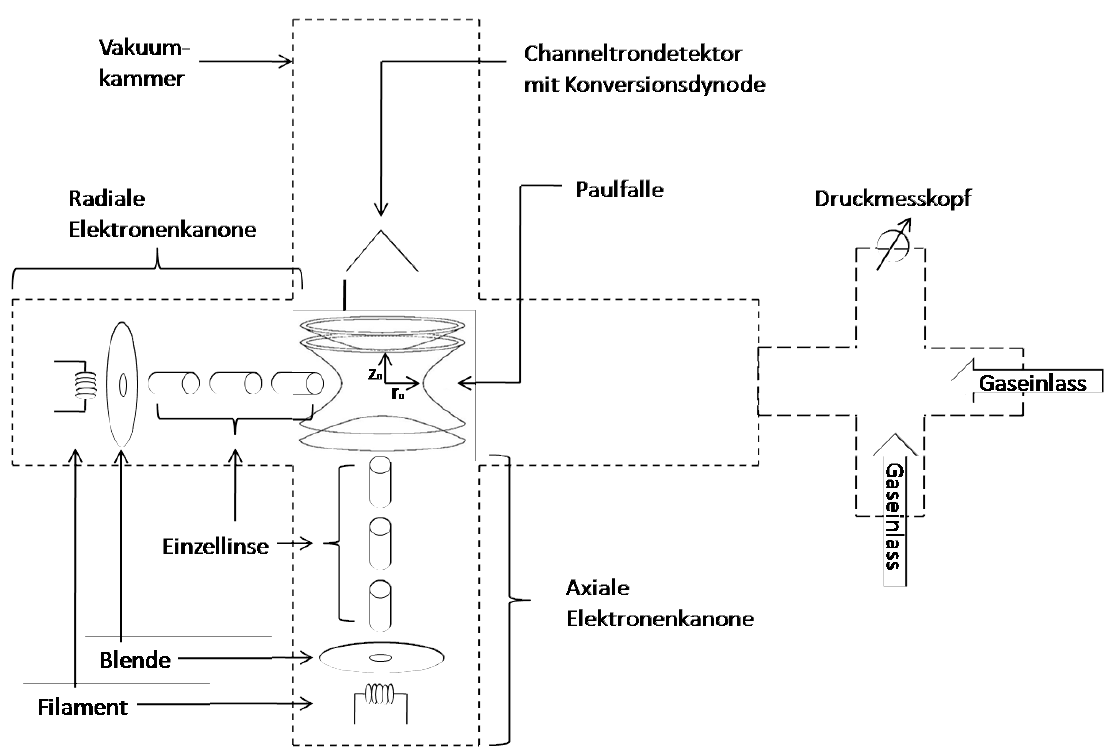
\includegraphics[width=0.7\textwidth]{aufbau.png}
				\caption{Schematischer Aufbau des Versuchs. \cite{EMAUGreifswaldPaul}}\label{img:aufbau}
			\end{figure}

	\clearpage
	\section{Auswertung}

		\subsection{Variation der Speicherzeit}

			Nachdem man sich mit dem Aufbau und der dazugehörigen Steuerung vertraut gemacht hatte, wurde ein Scan für die Speicherzeit in der Falle durchgeführt. Das heißt, dass die Zeit zwischen Ionisation (Elektronenkanone an) und Auswurf-Anregung durch den ersten Manipulationsgenerator variiert wurde. Die Ergebnisse sind in \autoref{img:zeit} zu sehen. Zu erwarten ist ein exponentielle Zusammenhang nach \tilt{Lambert-Beer}, da die kollektive Ionenbewegung und die Lebensdauerverteilung statistisch sind. Eine logarithmische Auftragung liefert die Bestätigung mit \autoref{img:lin}. Die 'Lebensdauer' bzw. die mittlere Verweildauer in der Falle bestimmte sich zu $\unit[5,1408]{ms}$.\\
			Eine Einzelmessung bestand jeweils als 10 'inneren' Iterationen, d.h. Messzyklen, welche in ihrer Intensität aufsummiert wurden. 50 äußere Iteration wiederholen den gesamten Vorgang von einer Wartezeit 0 bis $\unit[500]{\mu s}$ in chronologischer Reihenfolge, um eventuelle Zeitabhängige Fehler in der Messung zu eliminieren.

				\begin{figure}
					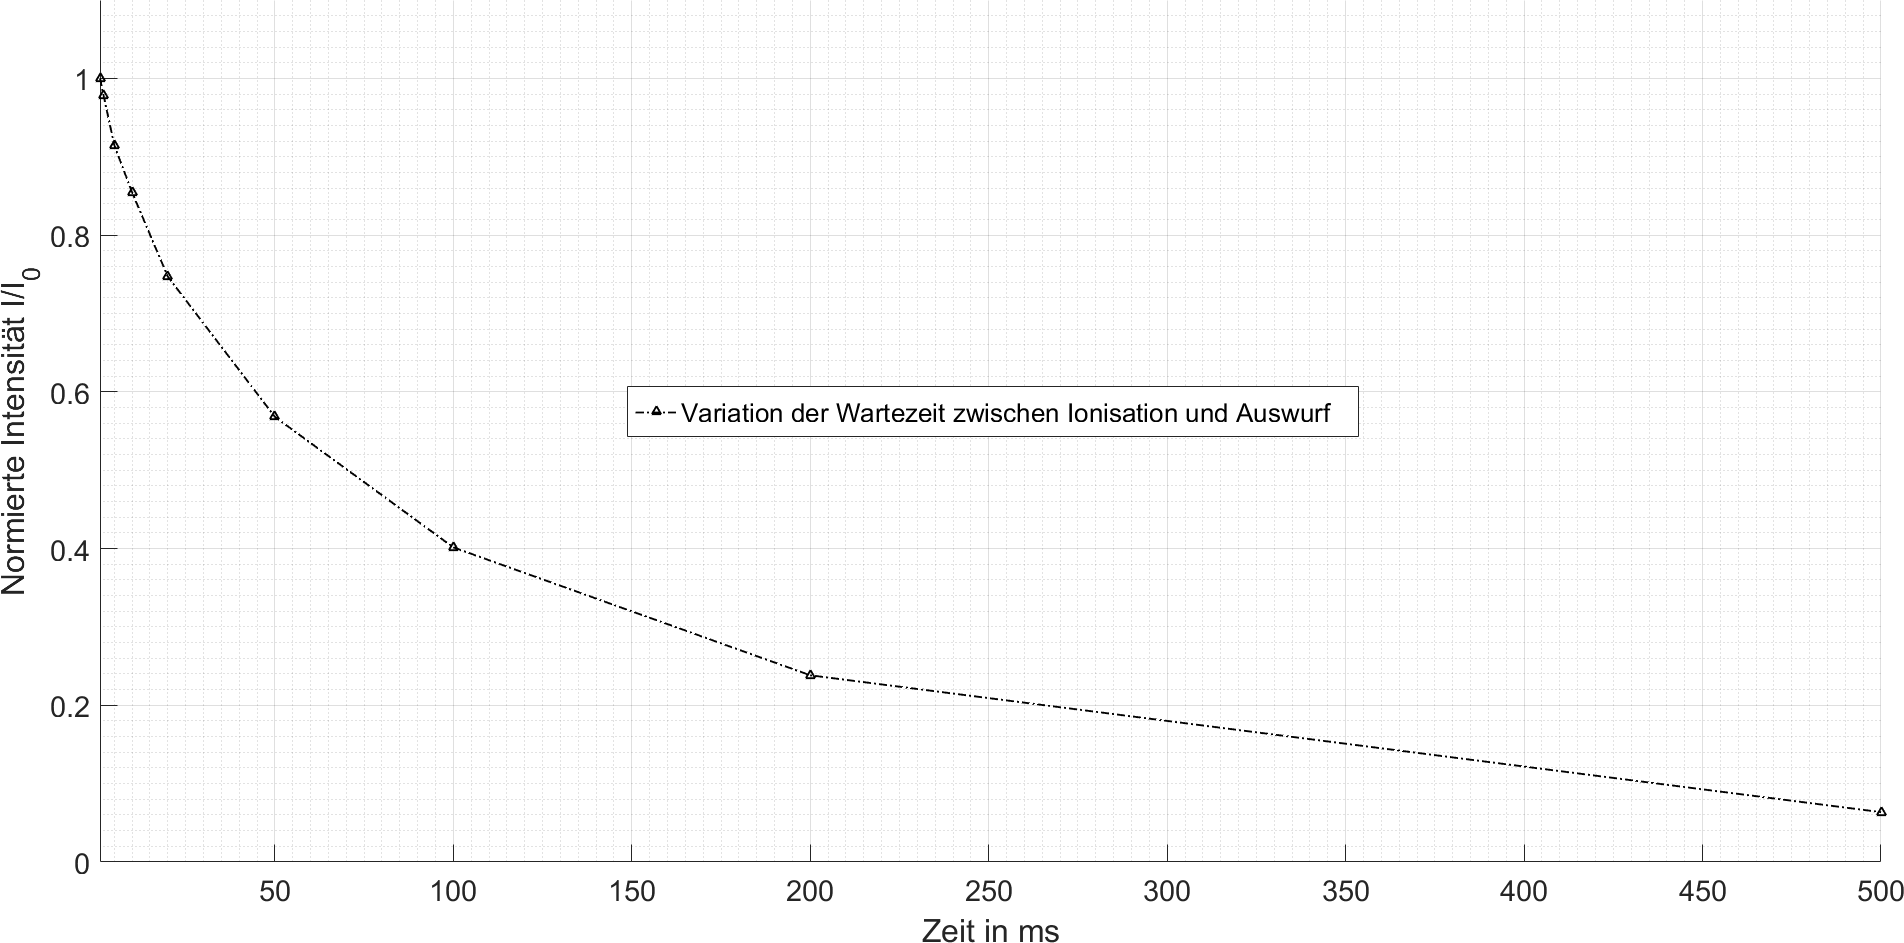
\includegraphics[width=\textwidth]{wartezeit.png}
					\caption{Norm. Signalintensität über Variation der Wartezeit zwischen Ionisation und Auswurf auf den Detektor.}\label{img:zeit}
				\end{figure}

				\begin{figure}
					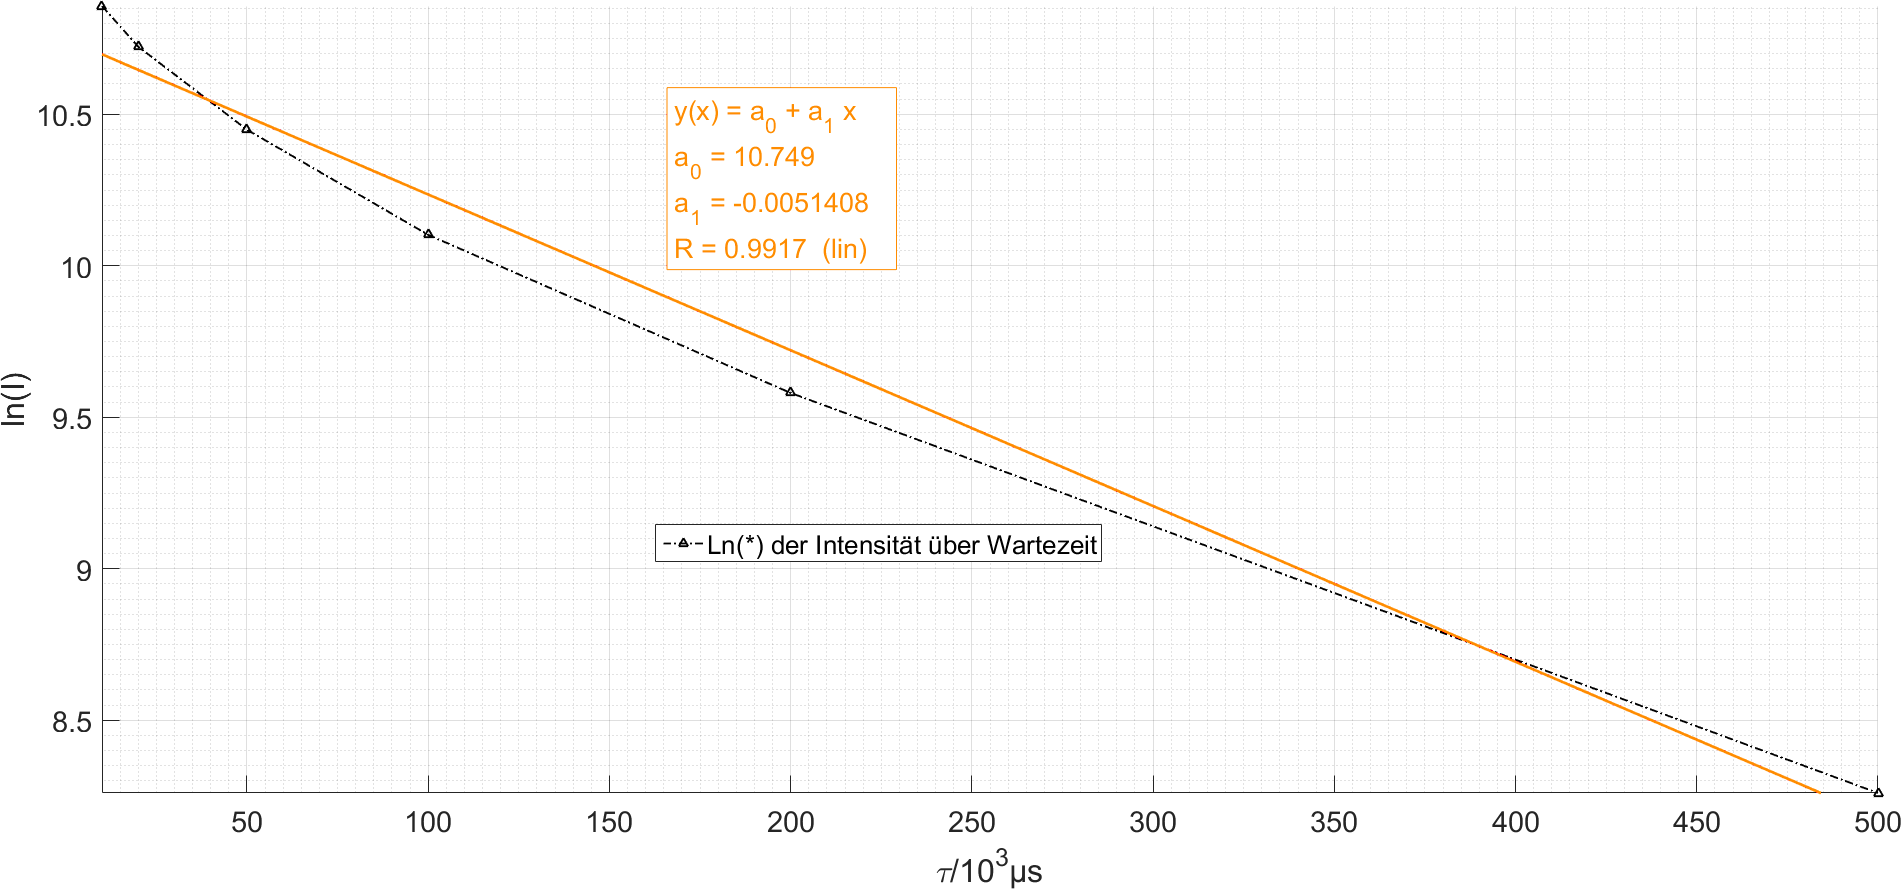
\includegraphics[width=\textwidth]{linear_fit_wartezeit.png}
					\caption{Fit eines Polynoms erster Ordnung an den Logartihmus der Intensität. Die erhaltene Funktion ist eingezeichnet. Der Koeffizient $a_1$ gibt die Lebens- oder Speicherdauer in Fall wieder.}\label{img:lin}
				\end{figure}

		\subsection{Frequenzvariation der primären Anregung}

			In dieser Messung wurde die Frequenz der primären Anregung zum Auswurf aus der Falle auf den Detektor verändert. Es wurde das gleiche Mess- und Datenaufnahmeprinzip wie zuvor verwendet. Die Messparameter sind insbesondere die selben. In $\unit[10]{kHz}$-Schritten wurde ein Bereich von $\unit[\tenpo{5}]{Hz}$ bis $\unit[5\cdot\tenpo{5}]{Hz}$ abgerastert. Das Ergebnis zeigt \autoref{img:auswurf}. Damit sind des weiteren die bereits verwendeten Einstellungen der Manipulation bestätigt, da sich ein deutliches, unter anderem auch globales Maximum der Intensität des Ionenstromes auf den Detektor bei $\unit[350]{kHz}$ findet. Außerdem sind Nebenmaxima - bei ca. $\unit[110]{kHz}$, $\unit[140]{kHz}$ und $\unit[210]{kHz}$ - zu sehen, wie sie von den Vorbetrachtungen vorhergesagt wurden. Auf die Untersuchung dieser zielt die nächste Messung ab (siehe \autoref{subsec:mess}).

				\begin{figure}
					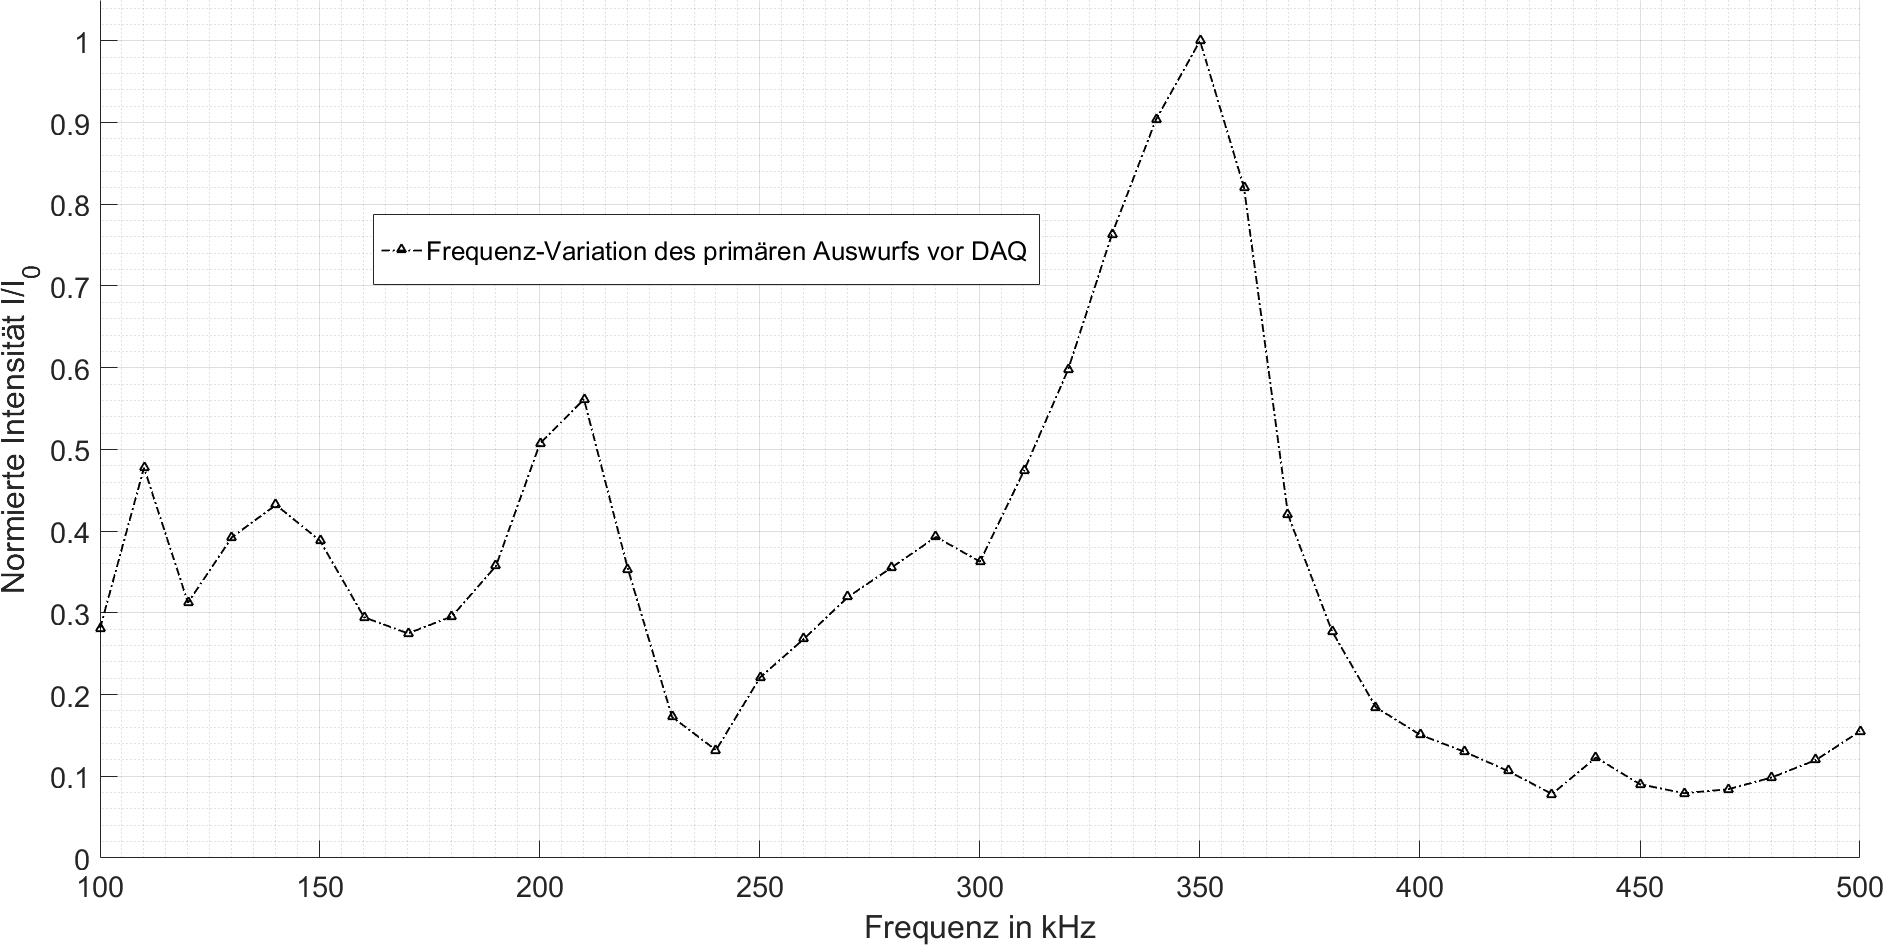
\includegraphics[width=\textwidth]{freq_auswurf.png}
					\caption{Signalintensität als Funktion der Frequenz des primären Auswurfs vor der Datenaufnahme. Strukturen sind deutlich, welche die Überlegungen der Grundlagen bestätigen und die Wahl einer Auswurf-Frequenz von $\unit[350]{kHz}$ nahe legen.}\label{img:auswurf}
				\end{figure}

		\subsection{Untersuchung der Eigenfrequenzen von ionisiertem Stickstoff}\label{subsec:mess}

			Bei dieser Messung ist es wichtig, das vollständige Spektrum der Anregung zu betrachten, da viele Frequenzen und deren lineare Kombinationen darin eingehen. Deswegen wurde ein Intervall von 0 bis $\unit[1,5]{MHz}$ gewählt, da bei der Führungsfeldfrequenz und in dessen Umgebung eine verstärkte Dynamik zu erwarten ist.\\
			Ein einzelner Zyklus startet mit der Elektronenka none für 10000\,µs, worauf eine sekundäre Manipulation mit dem Frequenzschritt $f\ix{n}$ für 1000\,µs folgt. Danach 'ruht' die Messung für weitere 10000\,µs, wobei die Ionen einfach in der Falle verweilen. Schließlich läuft für 2000\,µs die Datenaufnahme des Detektors zusammen mit der primären Anregung mit $\unit[350]{kHz}$. Für jeweils einen solchen Zyklus gibt es einen Referenzverlauf, welcher im Anschluss dazu jedoch ohne die sekundäre Anregung erfolgt. Dieser dient der Eichung und Fehlerminderung. Das Ergebnis für 10 innere und 50 äußere Iterationen bei einer Schrittweite von $\unit[1]{kHz}$ zeigt \autoref{img:bullshit}.\\
			Ziel dieser Messung ist es, die Ionenintensität in Abhängigkeit von der Anregungsfrequenz aufzunehmen, um daraus ein Spektrum für die Eigenfrequenzen der Ionen zu erhalten. Man erwartet einen Verlauf nach dem Vorbild von \autoref{img:referenz}, wobei jedoch anderen Parameter verwendet wurden \cite{Paul-FalleREF}. Das Signal als Differenz von Referenz und sekundärer Anregung erhält demnach ein lokales Minimum, wenn mit einer Resonanzfrequenz der Probesubstanz angeregt wurde. Für den primären Auswurf auf den Detektor stehen dann weniger Ionen zur Verfügung.

				\begin{figure}
					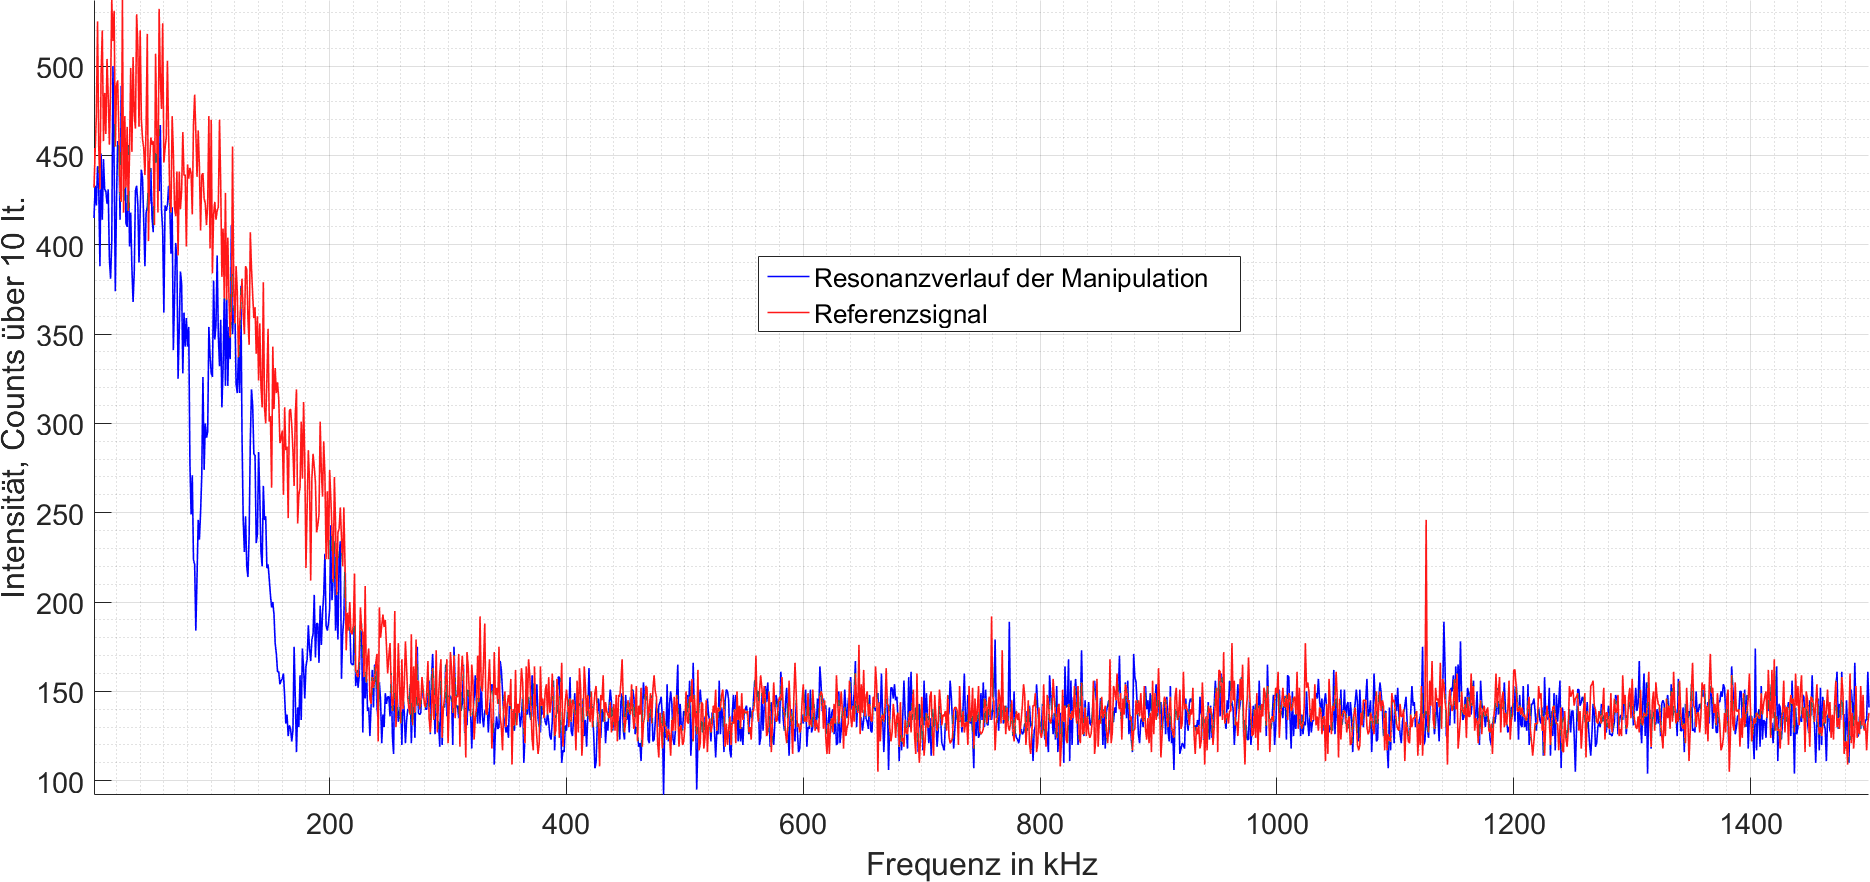
\includegraphics[width=\textwidth]{volle_daten.png}
					\caption{Frequenziteration einer sekundären Anregung in $1\,kHz$-Schritten bis $1,5\,MHz$. Volles Spektrum der 50 aüßeren und 10 inneren Iterationen.}\label{img:bullshit}
				\end{figure}

			Die \autoref{img:resonanz} - und außerdem \autoref{limg:1itsm} für die erste äußere Iteration bis $\unit[270]{kHz}$ - zeigt das letztendlich gesuchte Spektrum der Resonanzfrequenzen von $\fett{N}_2$-Ionen als die Differenz von Referenz- und Manipulationssignal.  Im Vergleich dazu ist der Verlauf aus \autoref{img:referenz} eingetragen, welcher für die selbe Ionensorte in \cite{Paul-FalleREF} aufgenommen wurde und hier als Literaturwert angenommen werden soll.\\
			Insgesamt scheint es so, als seien alle Resonanzen zu höheren Frequenzen verschoben worden. Angenommen dies sei der Fall, so wurden die Anregungen von $\omega_r$, $\omega_z$ und $\omega_z-\omega_r$ mit einem Fehler von $\pm\unit[20]{kHz}$ gefunden. Die ist aber insgesamt ein schwaches Kriterium, da bereits von einem Shift des gesamten Spektrums um etwa $+\unit[25]{kHz}$ auszugehen war. Eine Betrachtung der Fehler, welche konsequenter Weise aus dem Verlauf des Signals, insbesondere dem aus \autoref{img:bullshit} folgen, schließt sich im folgenden an.

				\begin{figure}
					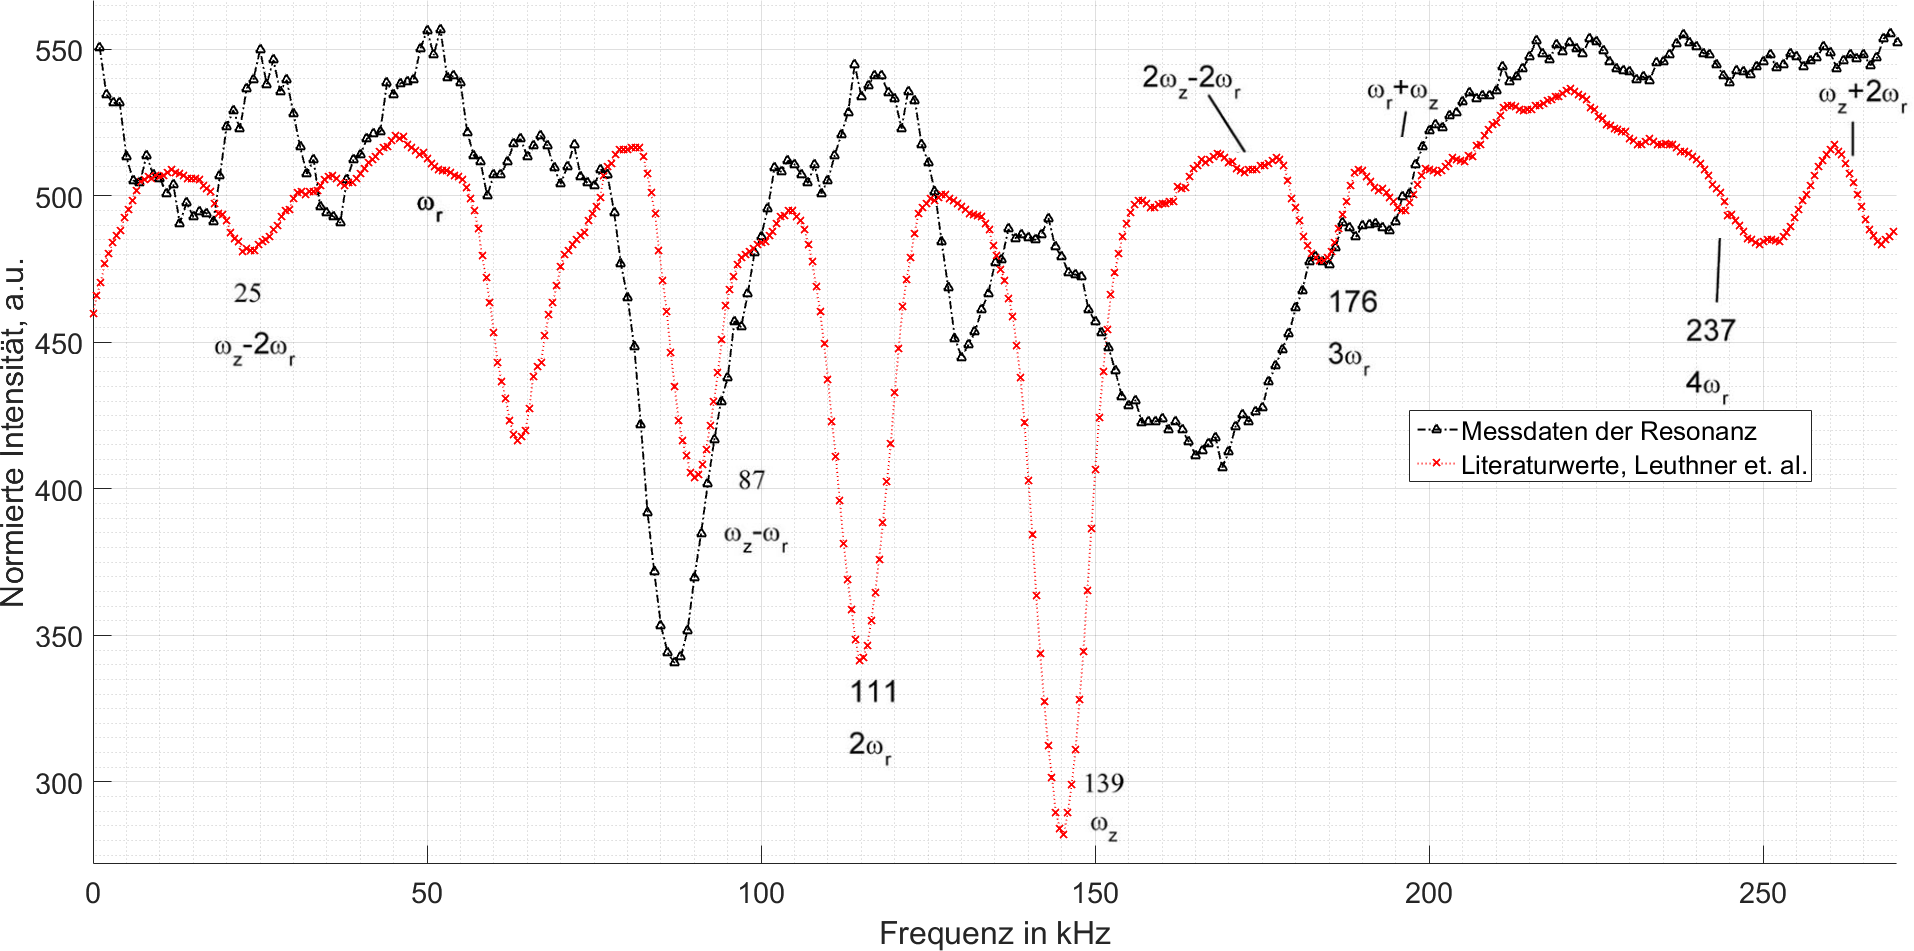
\includegraphics[width=\textwidth]{freq_diff_vergleich.png}
					\caption{Differenz von Referenz und Manipulation. Vergleich mit der Literatur \cite{Paul-FalleREF} bei geringfügiger Übereinstimmung.}\label{img:resonanz}
				\end{figure}

			Die \autoref{img:bullshit} vermittelt außerdem ein indiskutables Problem: das Messsignal ist nach $\sim\unit[300]{kHz}$ quasi nicht mehr existent und wird von da an nur noch von der Nullzählrate oder anderen zufälligen Ereignissen bestimmt. Es liegt der Gedanke nahe, dass bei dieser großen Messdauer das Experiment nach einer bestimmen Aufnahmedauer versagt hat. Deshalb zeigt \autoref{img:1it} die erste äußere Iteration im vollen Spektrum  - und \autoref{limg:1itsm} - , woraus durch einen Vergleich der Intensitäten ersichtlich wird, das bereits dort die vollständigen Informationen der Messung enthalten sind.

				\begin{figure}
				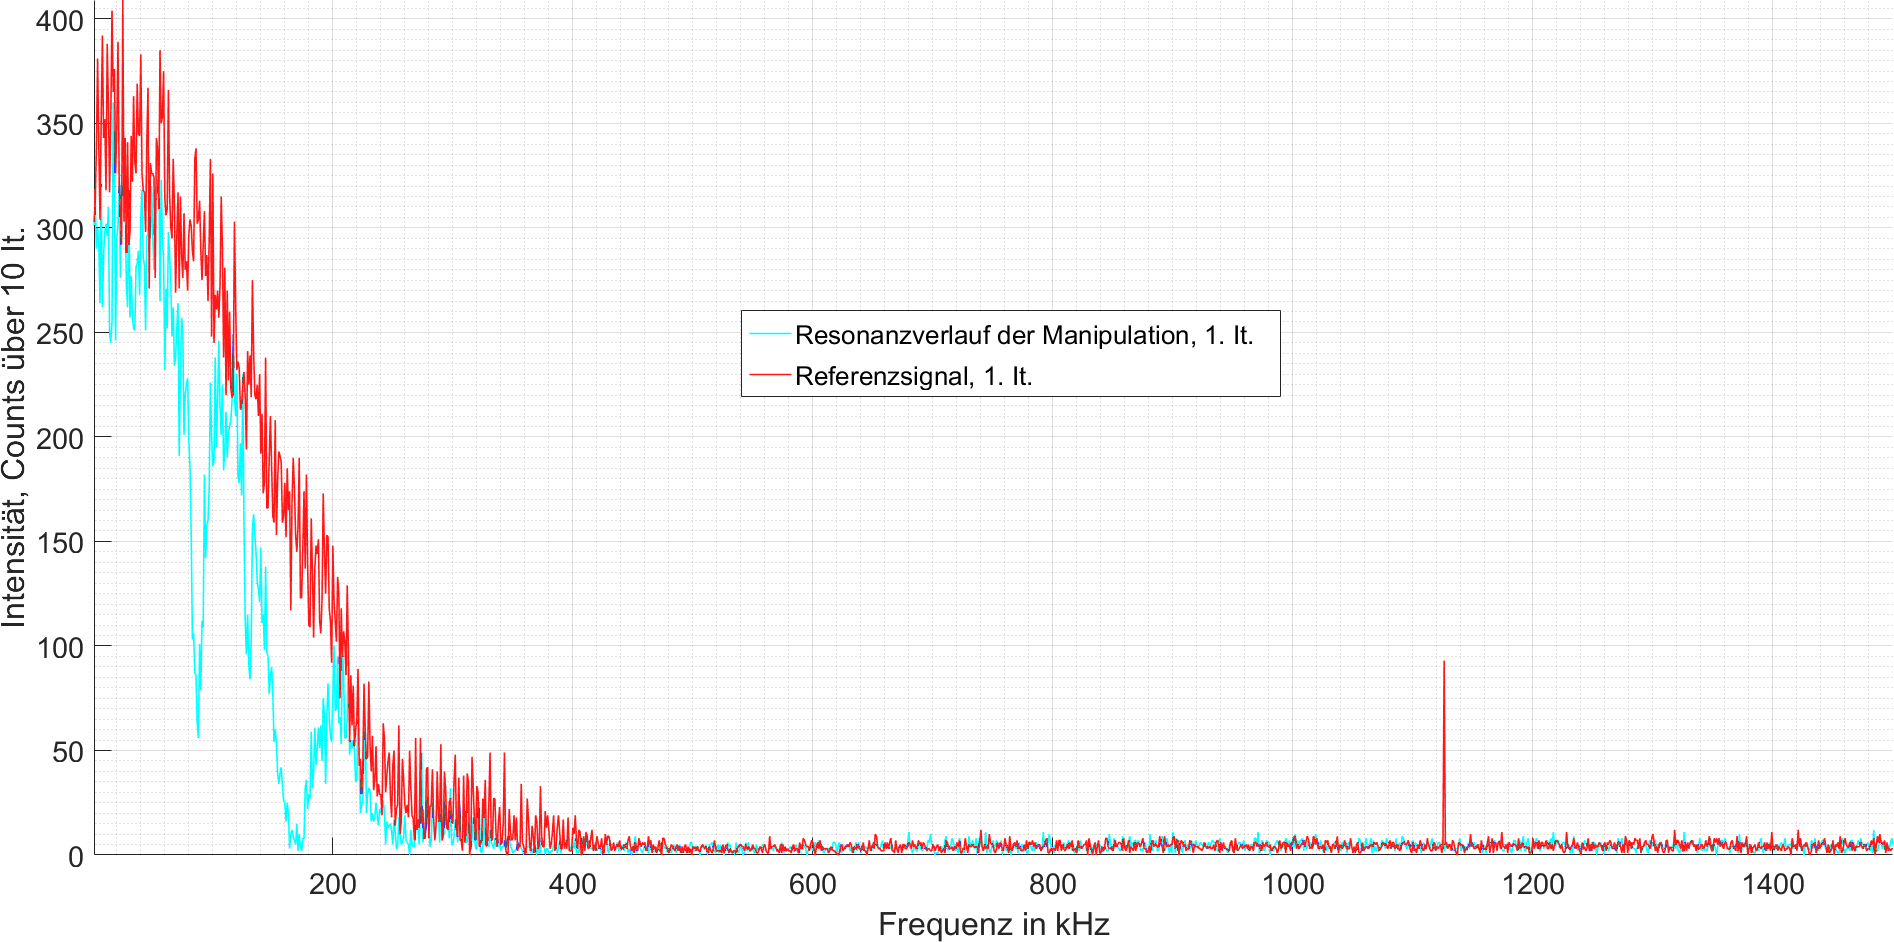
\includegraphics[width=\textwidth]{erste_it.png}
				\caption{Signal der ersten Iteration. Im Vergleich zum Vollen Spektrum erkennt man leicht, das hier die vollständigen, erhaltenen Daten stecken.}\label{img:1it}
				\end{figure}

				\begin{figure}
					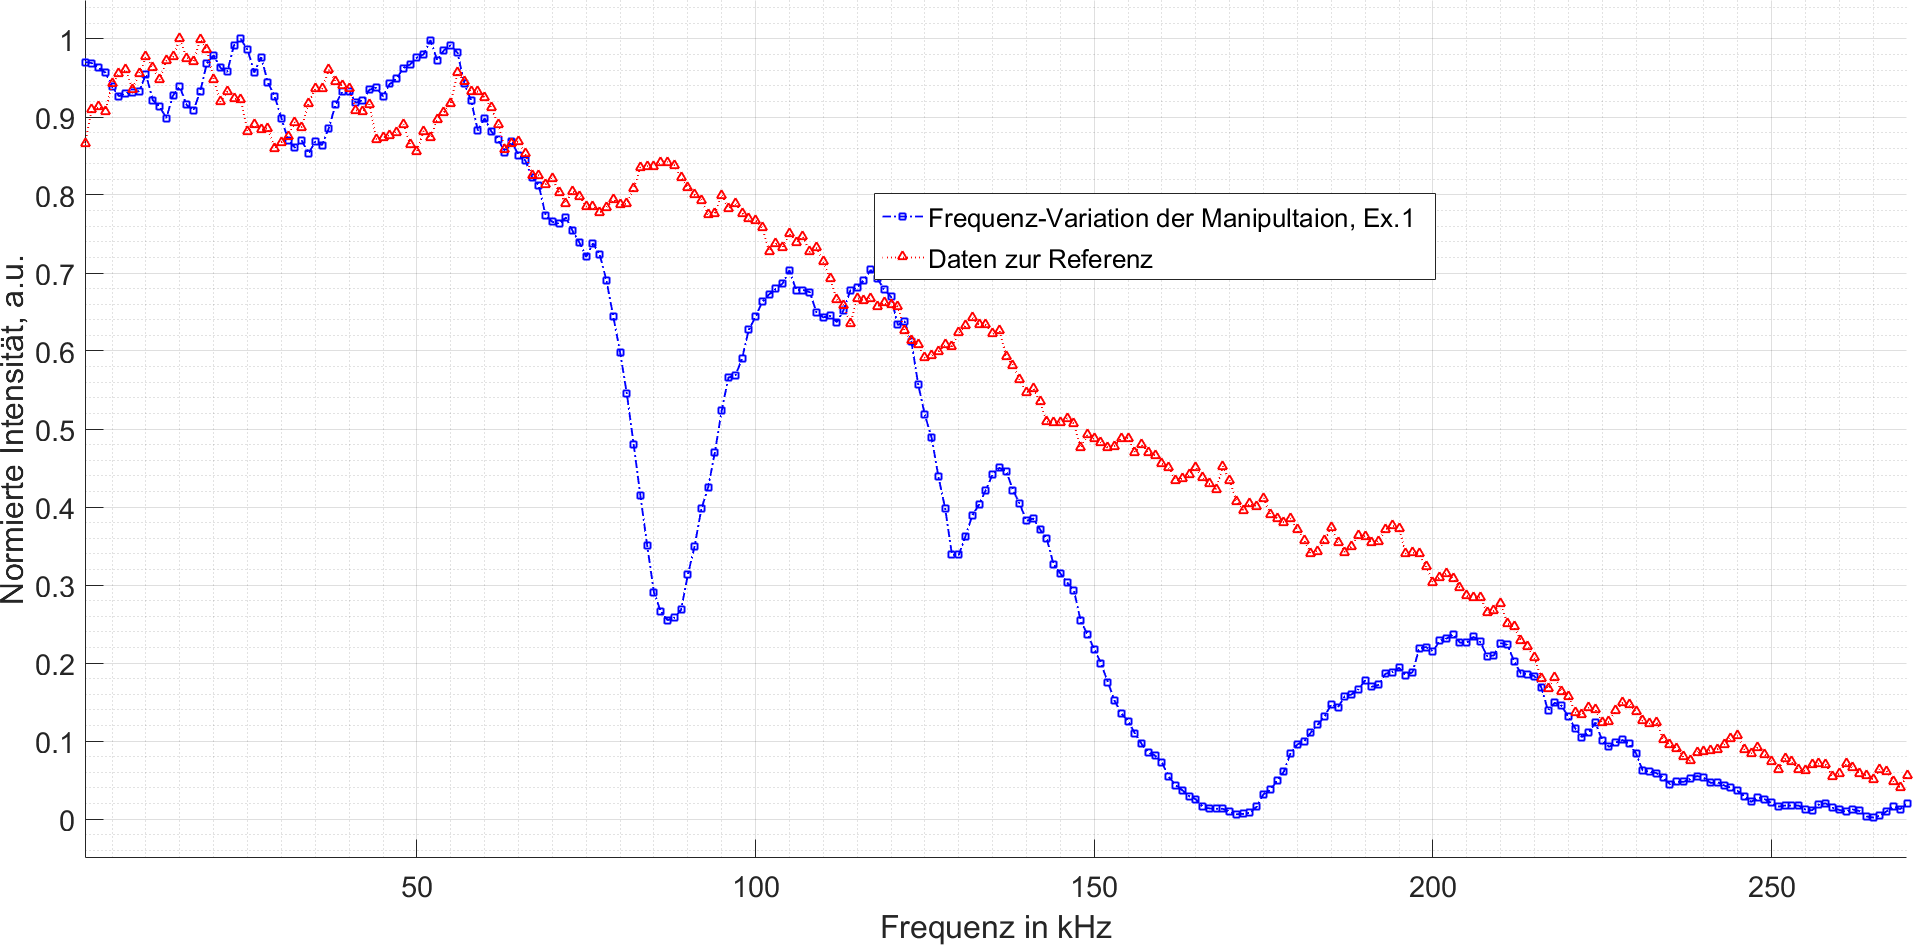
\includegraphics[width=\textwidth]{freq_smooth.png}
					\caption{Abfall der Signalstärke in Referenz und Manipulation. Unbearbeitete Daten für \autoref{img:resonanz}.}\label{img:1itsm}
				\end{figure}

			Nach dieser ernüchternden Erkenntnis wurde versucht, das Problem des Signalverlusts zu erkennen und zu beheben. Dafür betrachtete man das verbliebene Signal über der Experiment-Dauer. Wieder stehen dabei ein Manipulations- und ein Referenz-Zyklus im Vergleich: 10000\,µs E-Kanone für Ionisation, 1000\,µs sekundäre Anregung bzw. Warten, 10000\,µs Warten und 20000\,µs primäre Anregung mit Auswurf und Datenaufnahme. Der signifikante Unterschied zu vorherigen Messungen ist die, bei beiden Verfahren eingeführte Verweildauer von 50000\,µs nach der Detektor-Aufnahme - sozusagen als Pause des Experimentes zwischen Messungen. Ziel dabei war es, den möglichen Einfluss von Aufladungseffekten auf den Bauteilen und Raumladungen in der Falle zu minimieren. Die \autoref{img:abnahme} zeigt das Resultat von 50 äußeren und 10 inneren Iterationen.\\
			Bei einer anfänglich, bereits außergewöhnlich niedrigen Intensität von $\unit[207]{Cnts./10 It.}$ fällt das Signal mit rund $\unit[2]{Cnts./1000\,ms}$ ab. Nicht aber, dass dies nur der Fall für die sekundäre Anregung wäre, sondern auch für das Signal der Referenzmessung. Dies zeigt an, dass ein konzeptionelles Problem mit dem Aufbau bzw. der Falle selbst vorliegen muss. Weitere Messungen ergaben sich als nicht aussagekräftig, da bei nachfolgenden Zyklen das Signal sogar noch schwächer wurde oder sogar in das statistische Rauschen aus \autoref{img:bullshit} über ging. Im Rahmen dieses Praktikums und eines einzelnen Versuches über 2 Tage war es uns leider nicht möglich, tiefer greifende Fehleranalysen und Problembehebungen für die vorgestellten Hindernisse durchzuführen.

				\begin{figure}
					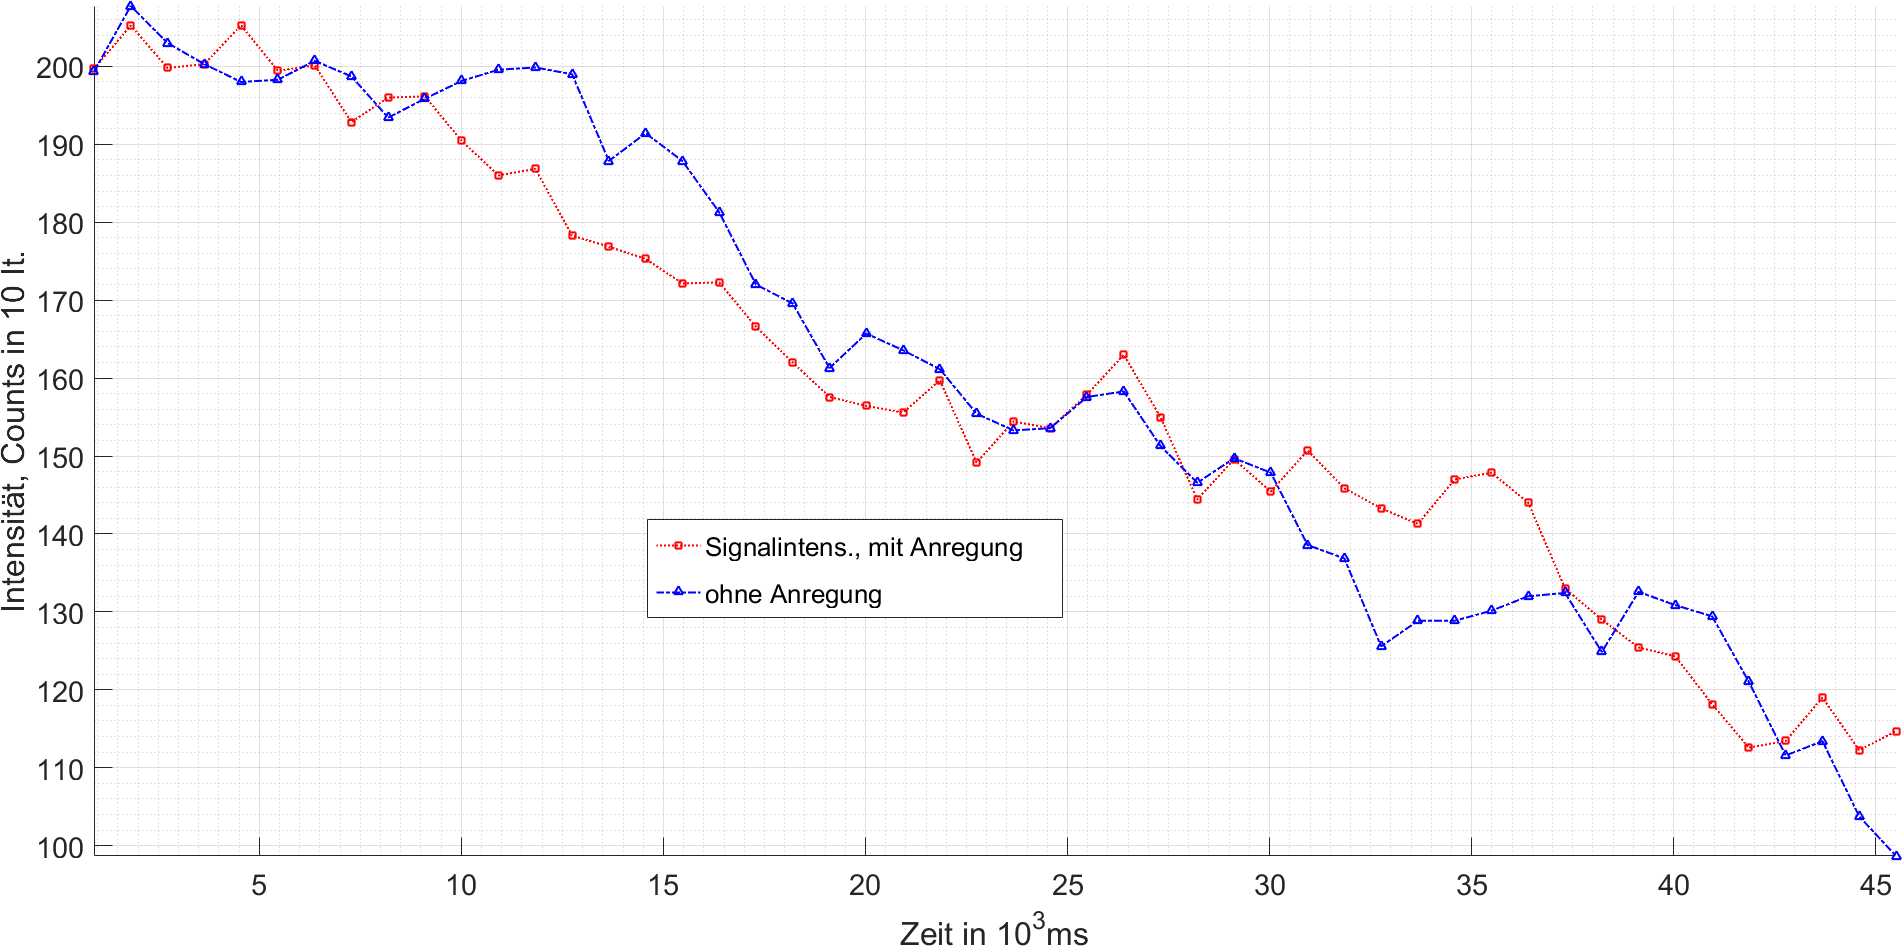
\includegraphics[width=\textwidth]{signal_abfall.png}
					\caption{Untersuchung des Intensitäts-Abfalls über der Experimentdauer. Sehr geringen Signalstärken gegenüber den Intensitäten aus \autoref{img:zeit}, welche im Bereich bon 5000-10000 lagen (dort nur normiert).}\label{img:abnahme}
				\end{figure}

	\clearpage
	\section{Anhang}

		\bibliography{all.bib}
		\bibliographystyle{unsrt}

\end{document}